\chapter{The Complete Quantum ALU}

By gathering the previous Quantum circuits we can create the Quantum Arithmetic Logic Unit very easily. Before
we do just that we would like to take a step back and analyse how this Unit may operate.

Just like a classical ALU, the Quantum ALU operates on some general purpose registers and on a register that stores
the status of logic operations. On top of those, the Quantum ALU, may need an \textit{operation code} or \textit{opcode}
to command it to do a specific operation. We shall analyze those opcodes further.

\section{The Quantum ALU's Opcodes}

We had introduced four different Quantum circuits in the previous chapters:
\begin{enumerate}
    \item a Quantum Adder-Subtractor,
    \item a Quantum Multiplier and
    \item a Quantum Comparator
\end{enumerate}
with each Quantum circuit giving us the operations of: addition, subtraction, multiplication and magnitued comparison.
We can encode these four operations using a bitstring of length $n=2$ because $log_24=2$. The mapping of each opcode with
its corresponding operation and Quantum circuit can be seen at the table below.

\begin{table}[ht]
    \centering
    \begin{tabular}{c|c|c}
        Opcode & Operation & Quantum circuit \\
        \hline
        \verb|00| & Addition & $QAS$ (Addition mode) \\
        \verb|01| & Subtraction & $QAS$ (Subtraction mode) \\
        \verb|10| & Multiplication & $QMUL$ \\
        \verb|11| & Magnitude Comparison & $QCMP_{NKO}$ \\
    \end{tabular}
    \caption{The Opcode table of the Quantum ALU}
\end{table}

\section{The Quantum ALU's circuit}

We will implement the Quantum ALU as any other Quantum circuit we have already presented. This Quantum circuit will have
in total sixteen qubits. The first two-qubit Quantum register is called the \textit{opcode} register and it stores the bitstring
of which operation the Quantum ALU must complete, the two two-qubit general purpose Quantum registers $A$ and $B$ is where
we store the binary encoded numbers we want to be operating, the eight-qubit output Quantum register $Out$ where it is used to
store the output of each operation and lastly, the two-qubit status Quantum register $Status$ where each qubit corresponds to
a logic flag.

\begin{figure}[ht]
    \centering
    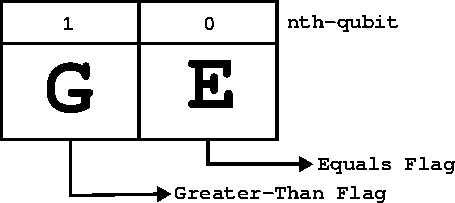
\includegraphics[scale=0.8]{images/6_Complete_System/status_reg_diagram.pdf}
    \caption{The diagram of the Status Quantum registers}
\end{figure}

\begin{listing}[ht]
    \centering
    \begin{minted}{python3}
        from qiskit import QuantumCircuit, QuantumRegister

        op = QuantumRegister(2, name="Opcode")
        a = QuantumRegister(2, name="A")
        b = QuantumRegister(2, name="B")
        out = QuantumRegister(8, name="Out")
        stat = QuantumRegister(2, name="Status")

        qalu = QuantumCircuit(op, a, b, out, stat)
    \end{minted}
    \caption{The initialization Python code for the Quantum circuit of the Quantum ALU}
\end{listing}

After the initialization of the circuit we have to append each of the Quantum circuits that implement each of the operations
as custom Quantum gates.

To control when each of the operation will be selected accordingly to the opcode bitstring we are going to use the member
method \verb|control()| of the \verb|Gate| class. This function takes numerous parameters but we are going to use only
two of those: the \verb|num_control_qubits| and the \verb|ctrl_state| parameters. The \verb|num_control_qubits| stores
how many qubits will be used control qubits to signal the activation of the gate and the \verb|ctrl_state| parameter
annotates what is the control state of each of the control qubits. For instance, the bitstring \verb|"101"| annotates
that the least-significant and most-significant qubits will be true when in the $\ket{1}$ state and the qubit in position
1 is going to be true in the $\ket{0}$ state (inverse logic).

Using this method it is very easy to map each gate/operation to the appropriate opcode bitstring: \\\verb|ctrl_state="10"| for
the multiplication gate and \verb|ctrl_state="11"| for the comparison gate. We just have to supply the opcode register
when appending.

The addition and subtraction operations where left last because they are not that straight-forward to append. These operations are
implemented by one gate that can change its mode by a control signal as an independent input. The other two operations needed
to set the \verb|num_ctrl_qubits=2| because they did not use a control signal as an input. This means that we can use one qubit
of the opcode register as an input for the Quantum Adder-Subtractor and thus we have to set \verb|num_ctrl_qubits=2| and
\verb|ctrl_state="0"| because according to the opcode table the most-significant qubit of the those operations is always in the
$\ket{0}$ state.

\begin{listing}[ht]
    \begin{minted}{python3}
        qalu.append(addsub.control(1, ctrl_state="0"),\
            ([op[1]] + [op[0]] + a[:] + b[:] + out[:n+1]))
        qalu.append(mul.control(2, ctrl_state="10"),\
            (op[:] + a[:] + b[:] + out[:]))
        qalu.append(cmp.control(2, ctrl_state="11"),\
            (op[:] + a[:] + b[:] + out[:n+1] + stat[:]))
    \end{minted}
    \caption{Appending the custom Quantum gates of the operations to the Quantum ALU}
\end{listing}

\begin{figure}[ht]
    \centering
    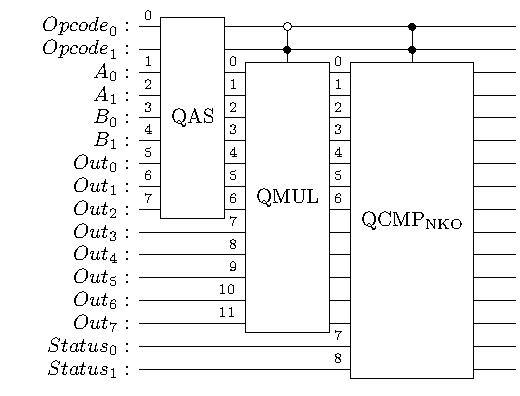
\includegraphics{images/6_Complete_System/qalu_complete.pdf}
    \caption{The Quantum circuit diagram of the Quantum ALU}
\end{figure}

\section{Running Examples on the Aer Simulator}

We will now demonstrate all of the operations of the Quantum ALU starting with addition and subtraction. Before executing the
Quantum circuit on a Aer simulator we will have to initialize the Opcode, A and B registers with the appropriate values. To
Let A and B be initialized with the unsigned values $3=11_2$ and $2=10_2$ accordingly. To perform an addition the Opcode
register must be initialized with the value $00_2$ and because every qubit in Qiskit is initialized with a $0$ by default
we do not need to explicitly set anything.

\begin{listing}[ht]
    \begin{minted}{python3}
        qalu.x(a[0])
        qalu.x(a[1]) # a = 11

        qalu.x(b[1]) # b = 10
    \end{minted}
    \caption{Initializing the Quantum registers A and B with appropriate values}
    \label{ls:6_init_add}
\end{listing}

Then after instanciating an Aer simulator, transpiling the Quantum circuit and executing it we get the following histogram:

\begin{figure}[ht]
    \centering
    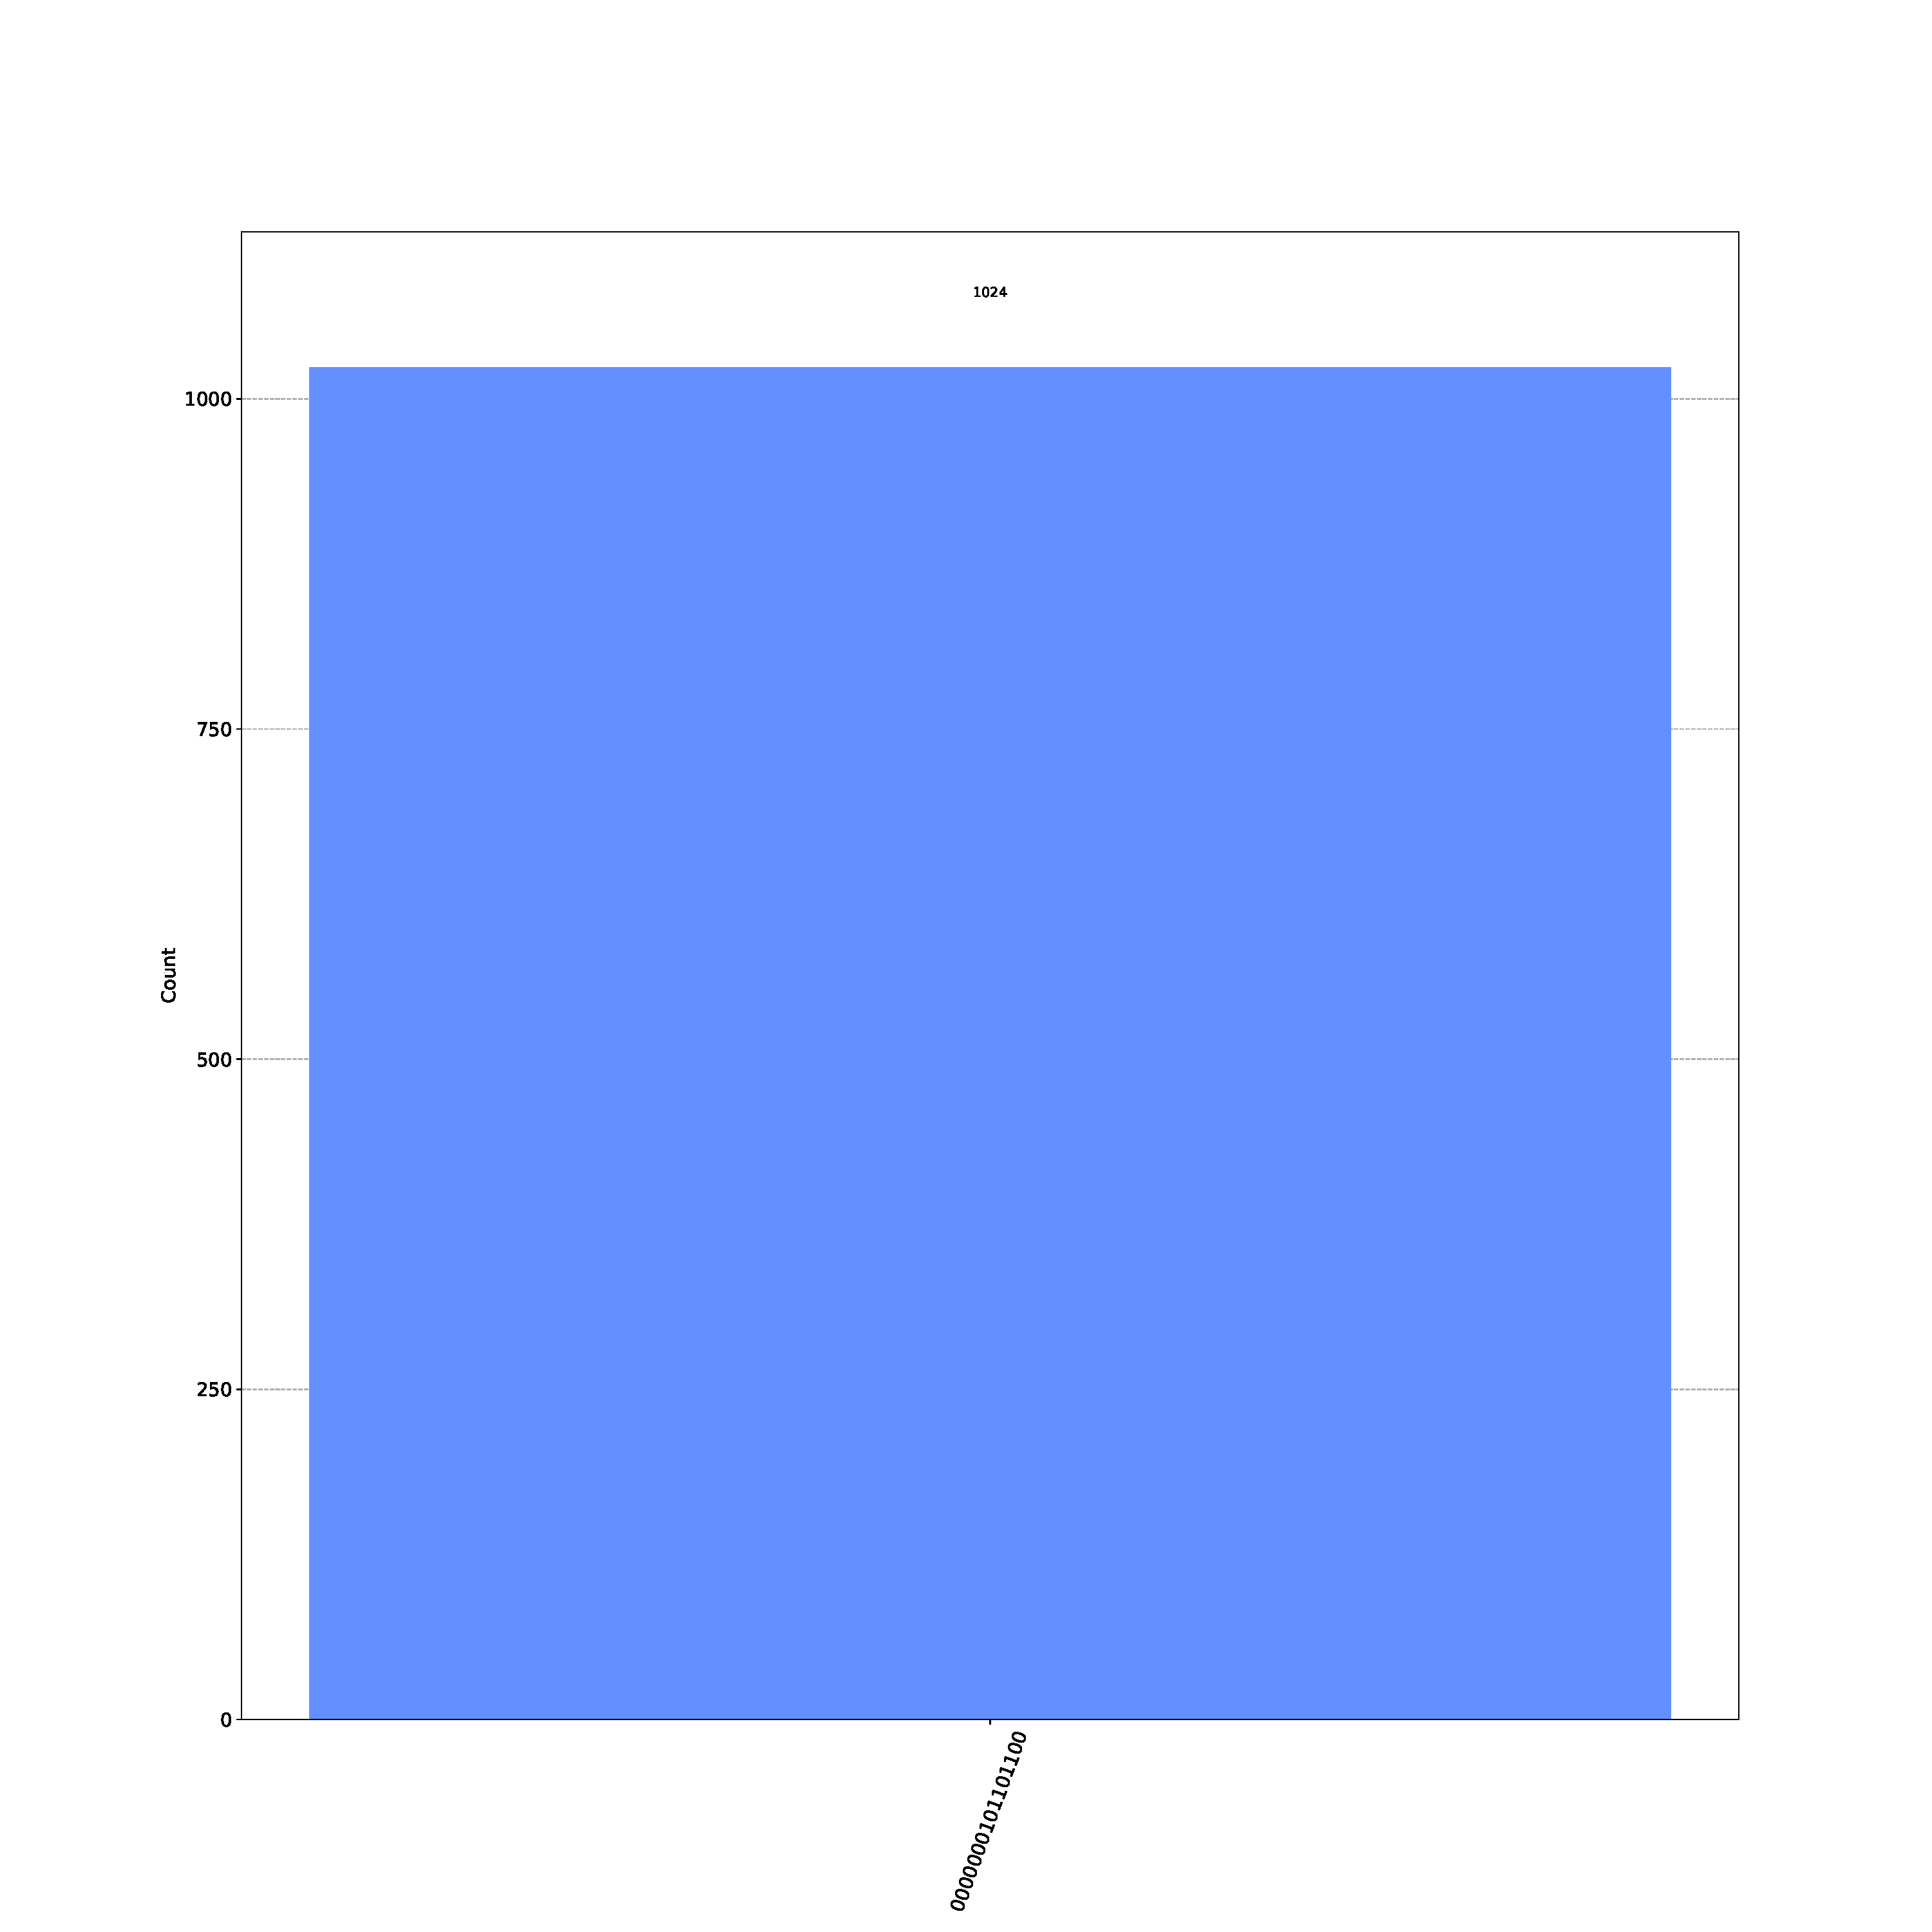
\includegraphics[scale=0.2]{images/6_Complete_System/qalu_aer_result_addition.pdf}
    \caption{The histogram of the result of the execution of the addition using the Quantum ALU}
\end{figure}

The most important data (for this kind of testing) is the label on the x-axis. This is a bitstring of the measurent outputs of the circuit after the 
addition operation. The measurement was invoked by the \verb|measure_all()| method which measures all qubits with the order
they are inputed when the Quantum circuit was instanciated but outputed in reverse. Then we first invert the output sequence:
$0000000101101100\mapsto001101101000000$. Then we seperate to match each Quantum register: $00$, $11$, $01$, $1010000$, $00$.
Finally, reverse the sequences once again: $00$, $11$, $10$, $0000101$, $00$. We could also make a table to visualize the contents
of each Quantum register after the execution of the Quantum circuit.

\begin{table}[ht]
    \centering
    \begin{tabular}{c|c|c|c|c}
        Opcode & A & B & Output & Status \\
        \hline
        $00$ (Addition) & $11$ ($3_{10}$) & $10$ ($2_{10}$) & $0000101$ ($5_{10}$) & $00$ (n/a)\\
    \end{tabular}
    \caption{The visualization of the contents of each Quantum register after the addition operation}
\end{table}

We can see that the output register that holds the binary value $101_2$ is also the expected answer of the addition of $A+B=11_2+10_2$.

We shall also demonstrate the multiplication of those values ($3$ and $2$). This time we have to initialize the Opcode Quantum register.
The sequence for doing the multiplication is $10$ so we have to initialize the Opcode Quantum register as follows:

\begin{listing}[ht]
    \centering
    \begin{minted}{python3}
        qalu.x(op[1]) # op = 10
    \end{minted}
    \caption{The initialization of the Opcode Quantum register to perform the multiplication}
\end{listing}

The other registers are initialized just like the Listing \ref{ls:6_init_add}. The resulted histogram is as follows:

\begin{figure}[ht]
    \centering
    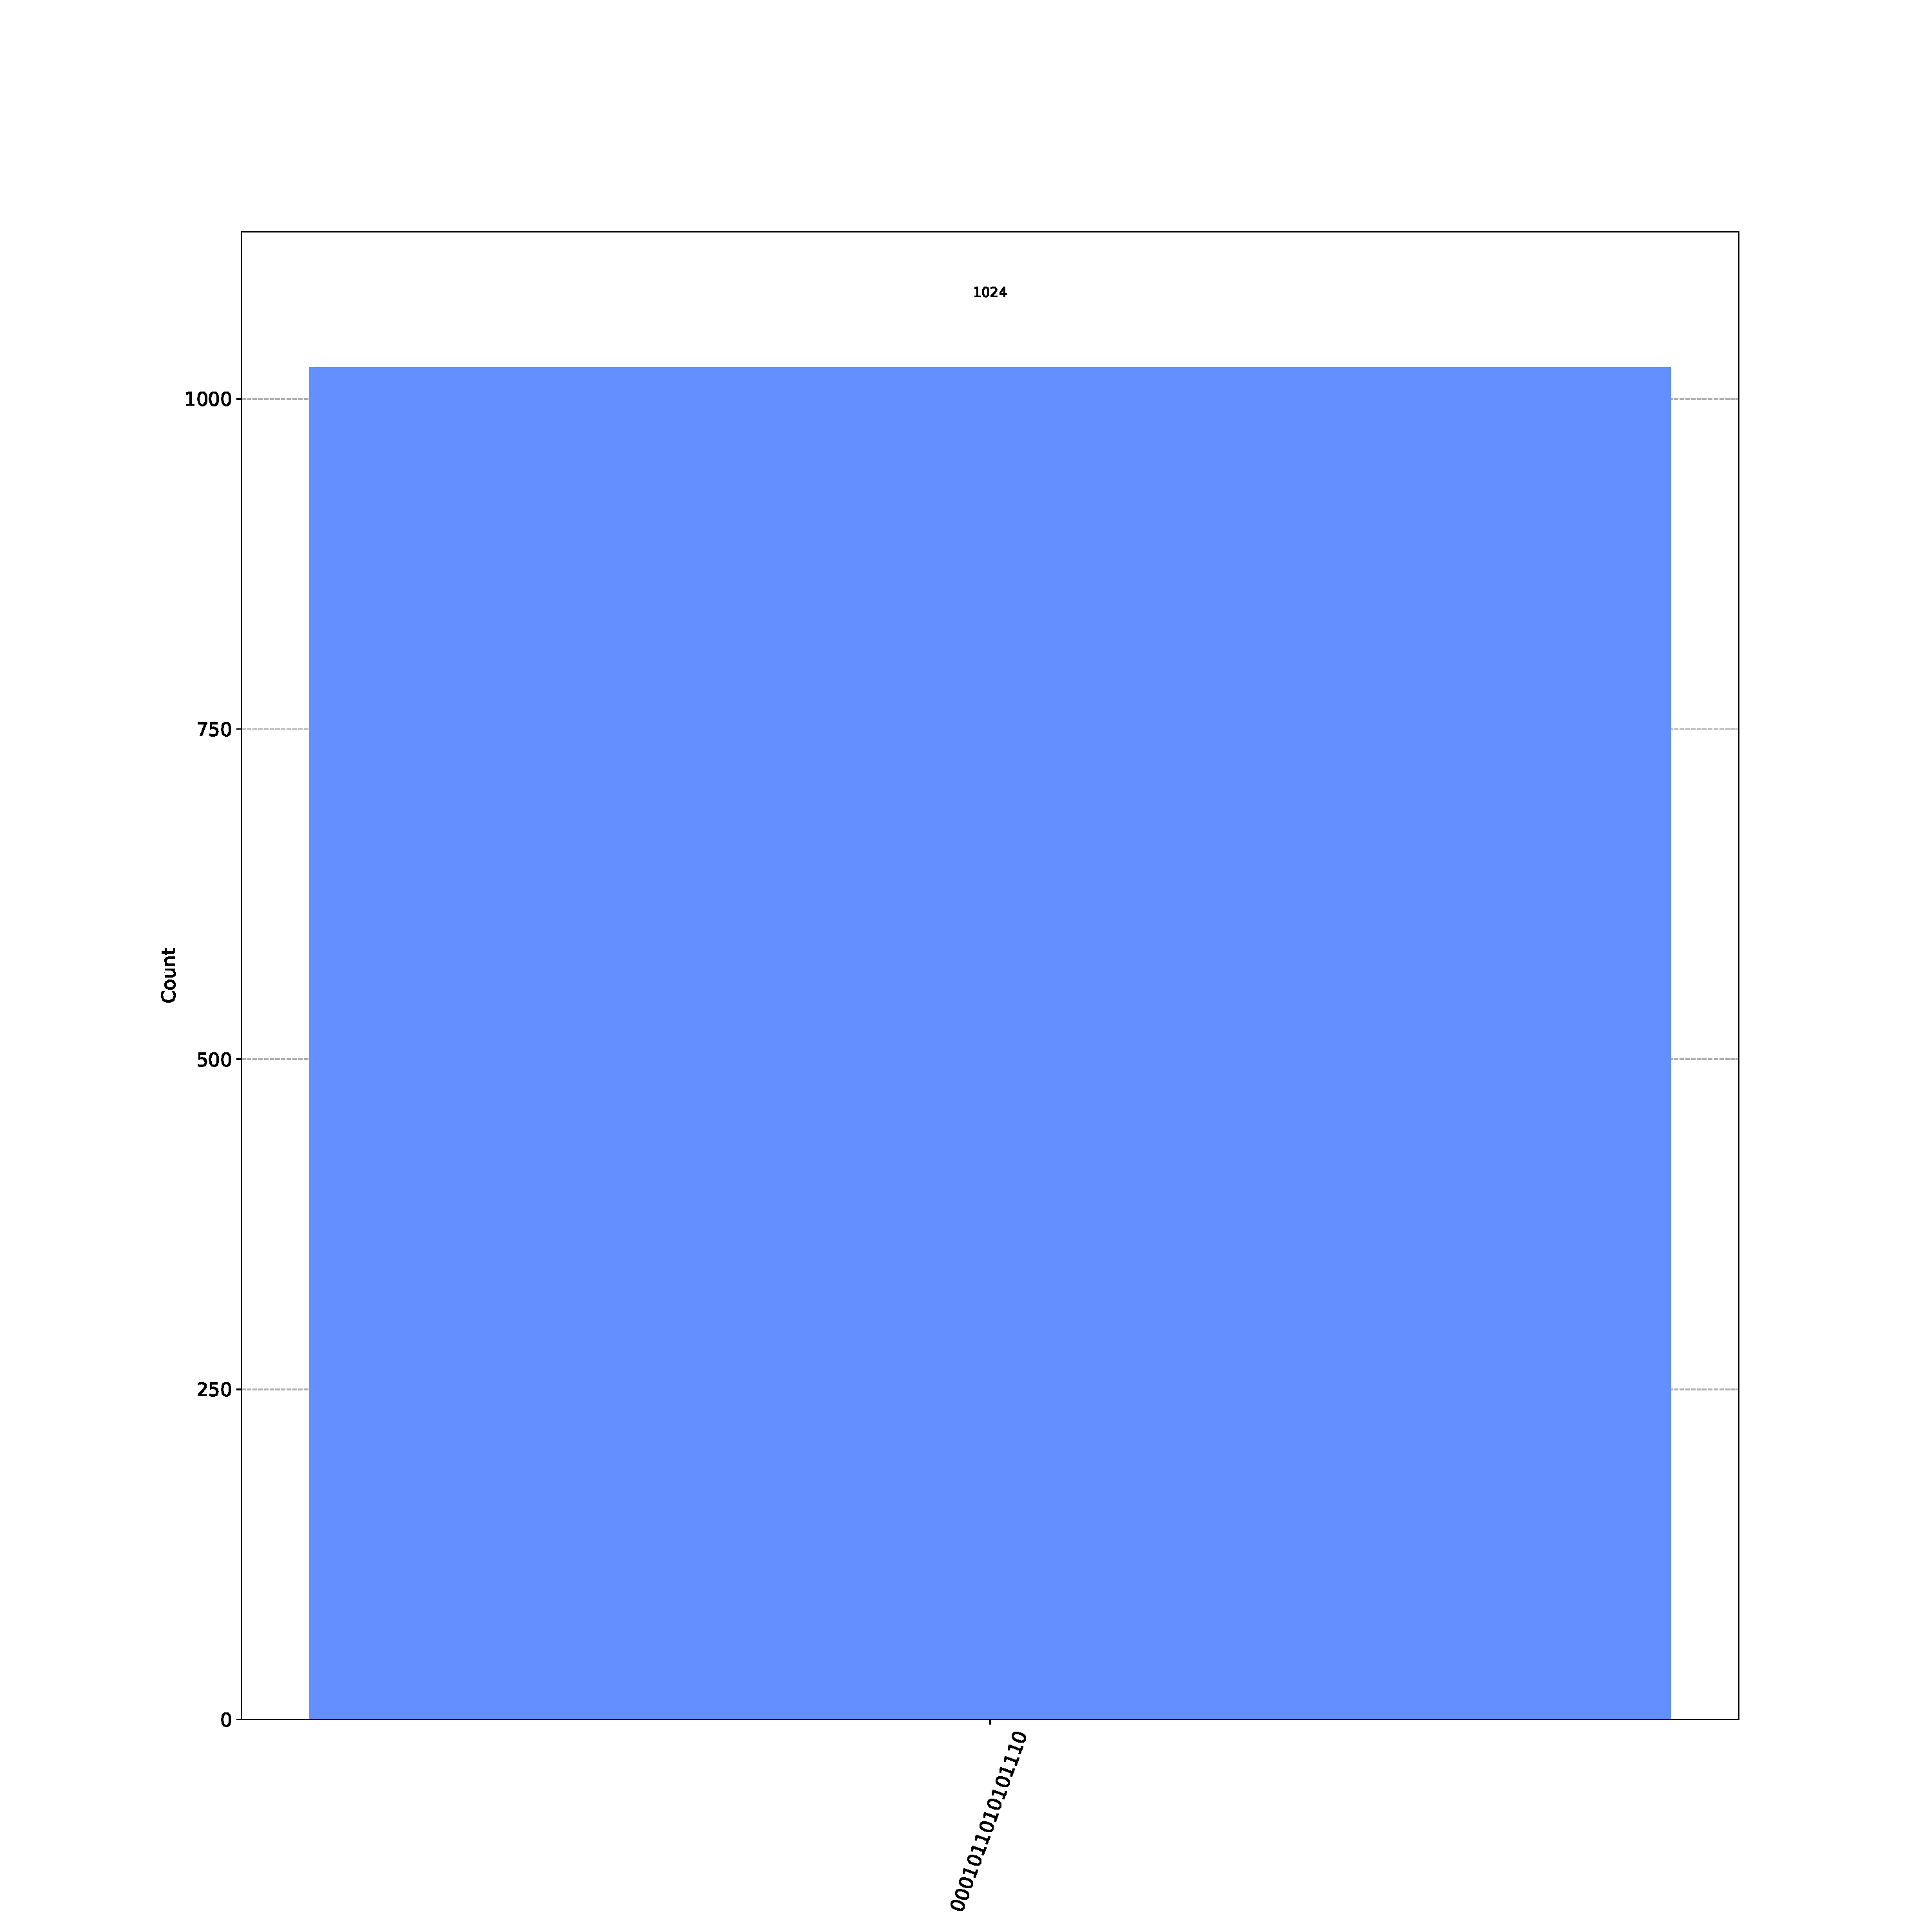
\includegraphics[scale=0.2]{images/6_Complete_System/qalu_aer_result_multiplication.pdf}
    \caption{The histogram of the result of the execution of the multiplication using the Quantum ALU}
\end{figure}

We repeate the simplification of the resulted data and we make the following table:

\begin{table}[ht]
    \centering
    \begin{tabular}{c|c|c|c|c}
        Opcode & A & B & Output & Status \\
        \hline
        $10$ (Multiplication) & $11$ ($3_{10}$) & $10$ ($2_{10}$) & $01011010$ & $00$ (n/a)\\
    \end{tabular}
    \caption{The visualization of the contents of each Quantum register after the multiplication operation}
\end{table}

To get the product of the values of the A and B Quantum registers we have to read only a specific subset of qubits of the Output Quantum register.
The qubits 0, 4, 6 and 7 store the product of the multiplication. Thus by reading only those qubits we create the sequence $0110_2$ which is what we expected.

\newpage

\section{Running Examples on Real Quantum Hardware}

We deliberately chose not to execute the subtraction and comparison operation on the Aer simulator so we could execute them on a real Quantum computer. Unfortunately, when
we send the two jobs to the IBM Quantum Platform, the platform warned us that the job's execution time would exceed the default ten minutes per month. For this reason we will
not send the entire circuit with the tuned inputs of each example but send two different circuits each implementing the appropriate operations. The only operations left for
demonstration are the subtraction and comparison which were analysed seperately in the previous chapter, thus we are going to use those circuits.

We are going to analyse the results of the subtraction of two two-qubit registers A and B, each initialized with the values $3=11_2$ and $2=10_2$ respectively. We 
measured the two qubits of the $C_{in}$ register (where the result of the addition-subtraction is held) and the only  qubits of the $C_{out}$ register (the overflow qubit).
We could have excluded the overflow qubit because the register A is greater in magnitude than the B register and when doing two's-complement subtraction we can exclude the
overflow but we kept it in to show that the circuit actually processes even the overflow of an operation.

\begin{figure}[ht]
    \centering
    \begin{subfigure}{0.5\textwidth}
        \centering
        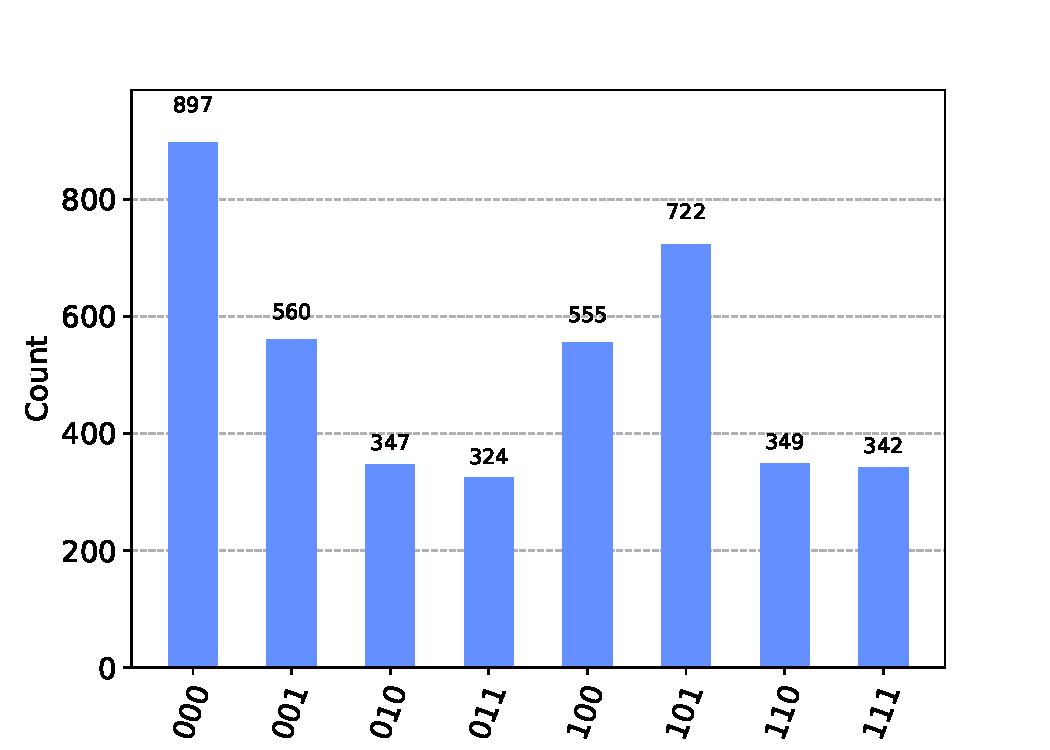
\includegraphics[scale=0.4]{images/6_Complete_System/adder_subtractor_ibmq_result.pdf}
        \caption{}
    \end{subfigure}
    \begin{subfigure}{0.5\textwidth}
        \centering
        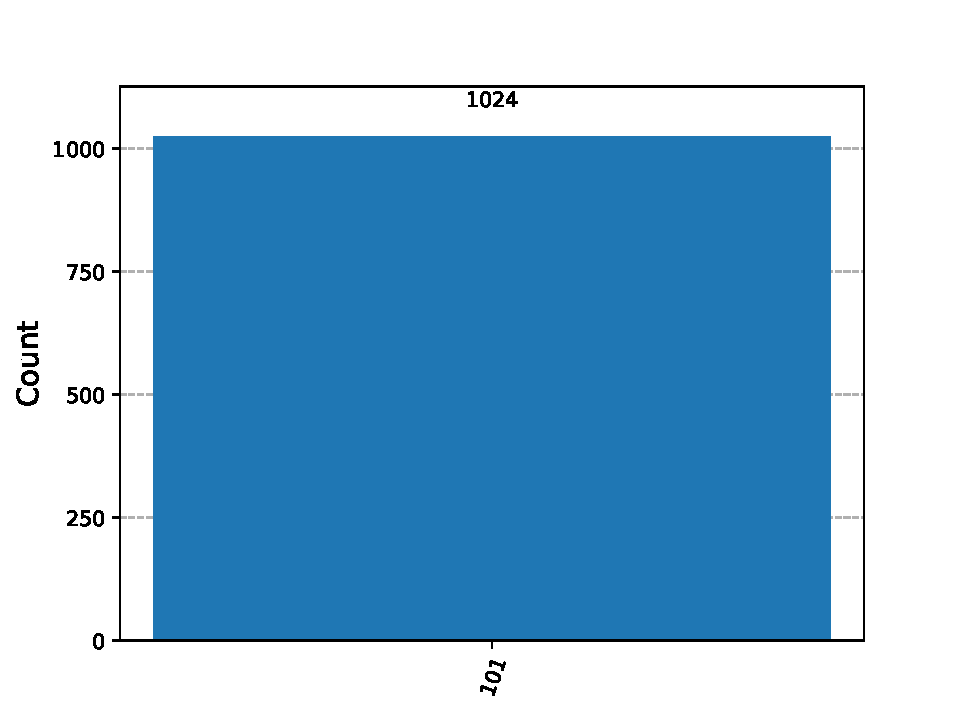
\includegraphics[scale=0.4]{images/6_Complete_System/adder_subtractor_aer_result.pdf}
        \caption{}
    \end{subfigure}
    \caption{The results  of the subtraction operation executed on the IBM Osaka (a) and on the Aer Simulator (b)}
\end{figure}

If we exclude the overflow qubit, the expected answer is $3-2=1$ or $01_2$ in binary. We can clearly see that the simulator, with $100\%$ certainty, the answer $101$ matches
the expected value. By contrast, in the histogram of the IBM Osaka execution, the output $101$ is the second most probable output, with a $17.6\%$ probability. The output
with most probability is the output of $000$, with a probability of $21.9\%$. We compiled a table with all the calculated probabilities, we note that any circuit executed on
an IBM Quantum Compute Resource has a default count value of $4096$, each circuit runs $4096$ times. We would also note that the probabilities where calculated using the
\verb|calc| arbitrary-precision terminal-based calculator on a Debian Linux distribution using the \verb|round()| built-in function and rounded on the nearest three decimal places.

\begin{table}[ht]
    \centering
    \begin{tabular}{c|c|c}
        Output Bit Sequence & Count & Probabilty ($\frac{\text{Count}}{4096}$) \\
        \hline
        $000$ & $897$ & $21.899\%$ \\
        $101$ & $722$ & $17.627\%$ \\
        $001$ & $560$ & $13.672\%$ \\
        $100$ & $555$ & $13.55\%$ \\
        $110$ & $349$ & $8.521\%$ \\
        $010$ & $347$ & $8.472\%$ \\
        $111$ & $342$ & $8.35\%$ \\
        $011$ & $324$ & $7.91\%$ \\
    \end{tabular}
    \caption{The result of probabilities of each output value of the execution of the subtraction operation on the IBM Osaka}
\end{table}

\newpage

On the other hand, we executed the NKO Comparator with the two two-qubit registers inputs A and B to be again $3$ and $2$ respectively and we only measured the two qubits
of the status Quantum register. The execution of the Quantum circuit happened on the IBM Osaka Quantum Computer too. We will again contrast the real-hardware result with the
simulation results.

\begin{figure}[!h]
    \centering
    \begin{subfigure}{0.5\textwidth}
        \centering
        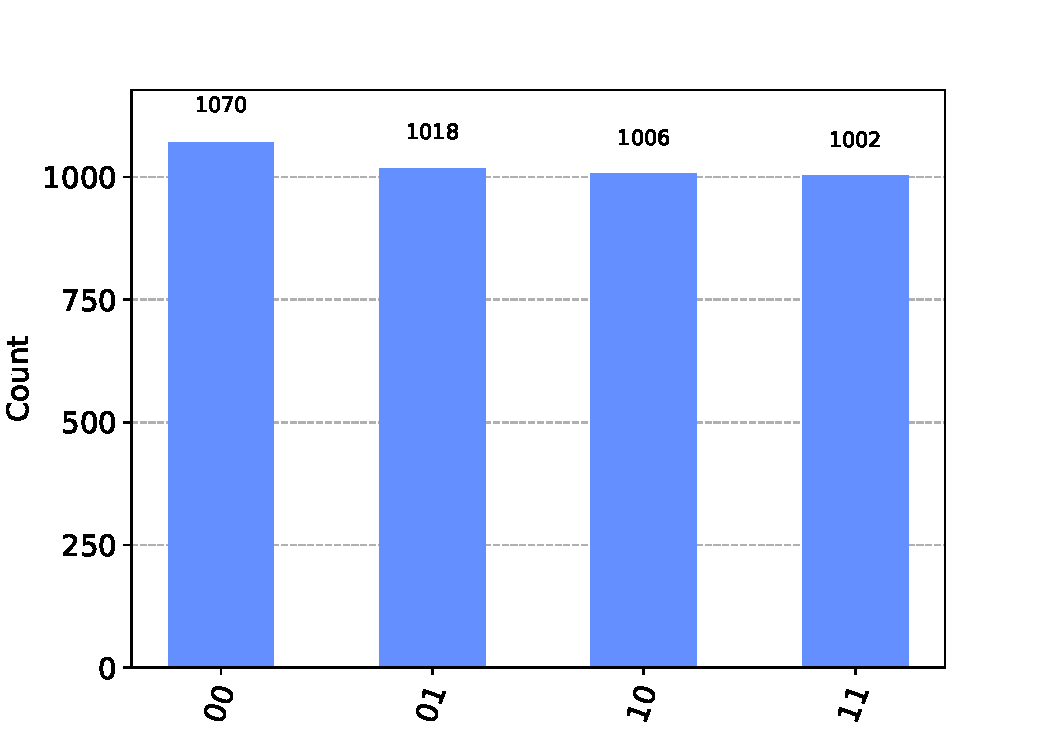
\includegraphics[scale=0.4]{images/6_Complete_System/nko_cmp_ibmq_result.pdf}
        \caption{}    
    \end{subfigure}
    \begin{subfigure}{0.5\textwidth}
        \centering
        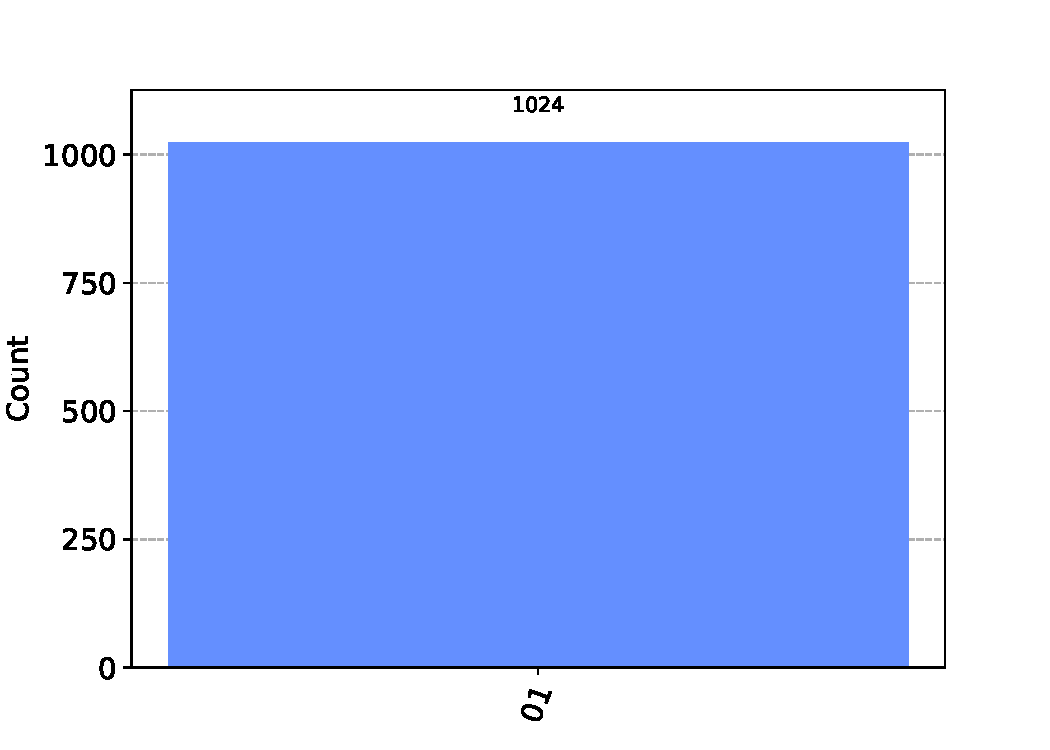
\includegraphics[scale=0.4]{images/6_Complete_System/nko_cmp_aer_result.pdf}
        \caption{}
    \end{subfigure}
    \caption{The results of the comparison operation executed on the IBM Osaka (a) and on the Aer Simulator (b)}
\end{figure}

The same story applies here, where the expected value, output'ed by the Aer Simulator, $10$ which means \say{$A\neq B\text{ and }A \geq B$}, is not the most probable output when executed
4096 times on the Quantum computer. We again compiled a table containing the probability of each output based on how many times the output occured while executing.

\begin{table}[ht]
    \centering
    \begin{tabular}{c|c|c}
        Output Bit Sequence & Count & Probabilty ($\frac{\text{Count}}{4096}$) \\
        \hline
        $00$ & $1070$ & $26.123\%$ \\
        $01$ & $1018$ & $24.854\%$ \\
        $10$ & $1006$ & $24.561\%$ \\
        $11$ & $1002$ & $24.463\%$ \\
    \end{tabular}
    \caption{The result of probabilities of each output value of the execution of the comparison operation on the IBM Osaka}
\end{table}

We can see that each output has relatively close probability of output meaning that the Quantum computer does not give us a reliable output.